% ===== 6. From probe to tokens: the Qwen3-1.7B refusal direction =====
\section{6. From probe to tokens: the Qwen3-1.7B refusal
direction}\label{from-probe-to-tokens-the-qwen3-1.7b-refusal-direction}

The probes of Section 5 certify that a refusal signal exists beyond prompt features. This section asks what the signal \emph{is}. I \emph{read} the direction through the model's own output head (§6.1), \emph{push} it onto real hidden states to test causation (§6.2), and \emph{take it apart} into sparse dictionary features to test which part carries the causal effect (§6.3).

% ----- 6.1 Probe-direction atlas: what the refusal signal points at in token space -----
\subsection{6.1 Probe-direction atlas: what the refusal signal points at
in token
space}\label{probe-direction-atlas-what-the-refusal-signal-points-at-in-token-space}

The refusal-vs-wrong probe at layer 28 carries the largest
baseline-adjusted margin of Table \ref{tbl:hadds}. Its weight vector
lifts back to raw hidden-state units,
\((\mathbf{w}_{\mathrm{raw}})_i = (V^\top w)_i / \sigma_i\) (PCA basis
\(V \in \mathbb{R}^{16 \times 2048}\), scaler stds \(\sigma\), sign
chosen so the refusal end is positive), and passes through the model's final RMSNorm and tied LM head:
\(\ell_v = \big[\mathrm{LMHead}(\mathrm{RMSNorm}(\mathbf{w}_{\mathrm{raw}}))\big]_v\)
for \(v \in \mathcal{V}\). RMSNorm is scale-invariant, so the \(\ell_v\) depend only on the direction. This is the same linear readout the head applies to any real state, so moving a state along the direction adds approximately these scores to its next-token logits, a prediction Section 6.2 confirms, with the lens scores as the \(\alpha \to \infty\) asymptote of the dose-response (calibration in Appendix C). One caution: this is \emph{epistemic} abstention expressed as a hedging opener, a different object from the \emph{safety}-refusal direction of \citet{arditi2024refusal}. The two need not coincide, and nothing here tests whether they do.

\textbf{Top tokens (full subset, \(n=549\)).} The ten highest-scoring
tokens are all tokenizations of ``as'', and the first non-``as'' token,
at rank 11, is \texttt{there}, the second-most-common refusal opening (scores in Appendix D.4). The refusals near-universally open with ``As of my knowledge cutoff in 2023\ldots{}'', so the probe is reading exactly that output-token commitment. An opener is a propensity, not a
guarantee, which is why the causal test scores the strict judge label
alongside the first-token rate. The confabulation pole shows no thematic
structure, and the layer-18 \emph{correctness} direction (all \(n=784\)
items) shows no comparable lens structure either (token detail in Appendix D.4). Section 6.2 tests its causal counterpart.

The n=393 within-post recovery (where every refusal actually lives) yields the same vocabulary in sharper form (Appendix D.4). With the within-post probe's \(+9.6\) pp margin (Section 5.6), the late-layer state carries a discrete pragmatic signal (``I am about to hedge'') not
extractable from the question text (score histograms in Figure
\ref{fig:score-hist}, Appendix D.4). A recovery-method check (Appendix
D.4, Figure \ref{fig:geometry}) shows the raw class-mean difference used
by safety-refusal work is \emph{not} this direction: it absorbs topical
and temporal-currency content where the probe concentrates the
register-and-opener component. In sum, this is a direction whose token-level signature is the refusal-opening vocabulary, a late-network commitment to a specific speech act, not a general ``self-knowledge'' representation.

% ----- 6.2 Causal validation by direct intervention -----
\subsection{6.2 Causal validation by direct
intervention}\label{causal-validation-by-direct-intervention}

The probe direction of Section 6.1 is \emph{correlational}. To test
whether it is also \emph{causal}, a forward hook adds
\(\alpha \cdot \mathbf{w}_{\mathrm{unit}}\) to the last prompt token's
post-block-27 residual during prefill on a stratified subset (30 wrong
post-cutoff + 30 refusal items), where \(\mathbf{w}_{\mathrm{unit}}\) is
the unit-normalized within-post recovery of Section 6.1 (hook detail in Appendix C). Generation passes through unmodified, one-shot at the moment of commitment. The perturbed residual is \emph{not} the cached normed state the probes read (Section 4). A coordinate-dissociation check refitting the probe natively on pre-norm residuals finds equal
discriminative accuracy but half the causal leverage (Appendix C), so
the normed representation, one linear map from the output head, is where
the potent direction lives. RMSNorm sets the natural \(\alpha\) scale, and working doses run from a third of the pushed state's own norm to about twice it (dose ratios and calibration scan in Appendix C). \textbf{Sweep:} \(\alpha \in \{-2000, -500, 0, 500, 1500, 3000\}\) on the 60 items, greedy, re-judged three-way. Outcomes are the strict judge-label refusal rate and a first-token refusal-opener rate over the Section 6.1 opener set (listed in Appendix C). The opener rate is
deliberately a first-token \emph{proxy} (an ``As\ldots{}'' opening does
not commit the model to refusing), which is why both measures are
reported and diverge.

\begin{table}[!htbp]
\small
\centering
\caption{The steering matrix: outcome rates for one-shot pushes along
the refusal direction, doses as fractions of the mean pre-norm state
norm ($\|\bar{\mathbf{h}}\| \approx 1640$; sweep
$\alpha \in \{-2000, -500, 0, +500, +1500, +3000\}$); $n = 30$ per
subset. Judged CORRECT stays $0\%$--$10\%$ on the wrong subset and
judged REFUSAL $\le 14\%$ on the correct subset throughout, for every
direction; the small judged-REFUSAL rates at negative doses on wrong
items ($\le 13\%$, $0\%$ opener rate) are sign-inconsistent magnitude
artifacts, not directional effects.\label{tbl:alpha}}
\begin{tabular}{@{}
  >{\raggedright\arraybackslash}p{(\linewidth - 14\tabcolsep) * \real{0.2394}}
  >{\raggedright\arraybackslash}p{(\linewidth - 14\tabcolsep) * \real{0.3380}}
  >{\raggedleft\arraybackslash}p{(\linewidth - 14\tabcolsep) * \real{0.0704}}
  >{\raggedleft\arraybackslash}p{(\linewidth - 14\tabcolsep) * \real{0.0704}}
  >{\raggedleft\arraybackslash}p{(\linewidth - 14\tabcolsep) * \real{0.0704}}
  >{\raggedleft\arraybackslash}p{(\linewidth - 14\tabcolsep) * \real{0.0704}}
  >{\raggedleft\arraybackslash}p{(\linewidth - 14\tabcolsep) * \real{0.0704}}
  >{\raggedleft\arraybackslash}p{(\linewidth - 14\tabcolsep) * \real{0.0704}}@{}}
\toprule
original label & metric & $-1.2\times$ & $-0.3\times$ & $0$ & $+0.3\times$ & $+0.9\times$ & $+1.8\times$ \\
\midrule
WRONG & opener rate & $0\%$ & $3\%$ & $10\%$ & $50\%$ & $97\%$ & $100\%$ \\
 & judged REFUSAL & $10\%$ & $0\%$ & $0\%$ & $13\%$ & $30\%$ & $30\%$ \\
\midrule
REFUSAL & opener rate & $0\%$ & $23\%$ & $100\%$ & $100\%$ & $100\%$ & $100\%$ \\
 & judged REFUSAL & $17\%$ & $40\%$ & $100\%$ & $100\%$ & $100\%$ & $100\%$ \\
 & judged WRONG & $77\%$ & $53\%$ & $0\%$ & $0\%$ & $0\%$ & $0\%$ \\
\midrule
CORRECT & opener rate & $0\%$ & $0\%$ & $0\%$ & $10\%$ & $63\%$ & $100\%$ \\
 & judged CORRECT & $93\%$ & $100\%$ & $100\%$ & $87\%$ & $57\%$ & $53\%$ \\
 & judged WRONG & $7\%$ & $0\%$ & $0\%$ & $7\%$ & $30\%$ & $33\%$ \\
\bottomrule
\end{tabular}
\end{table}

Table~\ref{tbl:alpha} is the steering matrix. Pushed toward refusal,
wrong items open with refusal vocabulary almost without exception from a
\(0.9\times\) dose, yet only a third of full generations convert: the
autoregressive continuation pulls back to content. Pulled away, refusing items collapse into attempts that are overwhelmingly confabulations. Correct items are untouched by the pull and largely resist the push, about half still delivering the fact through a forced refusal opening.
Suppressing the refusal decision does not unlock knowledge, and pushing
toward refusal does not reliably erase it: the direction gates the
opening speech act, and whether the fact is present decides what
follows. The matrix is a property of the refusal axis, not of one recovery. Rerun with the SAE-2191 and directly optimized directions, it reproduces the same plateaus row for row (parity block, Table \ref{tbl:alphaparity}, Appendix C).

\textbf{Interpretation.} The direction is a causal handle on the
refusal-opening \emph{readout}: it localizes where the commitment is
written, not the upstream circuitry computing it (transported
earlier-layer pushes are future work). The full outcome is \emph{co-determined} by autoregressive dynamics the one-shot push does not touch: a model can open ``As of 2024\ldots{}'' and still commit to a fact, hence the \(30\%\) vs.~\(100\%\) gap on wrong items. The reverse direction is stronger because the natural refusal trajectory is itself committed. A prefix-forcing control (Appendix C) reproduces the
judge-label outcome without touching the hidden state: the direction
causally selects the first token, and everything after token one is
ordinary autoregressive dynamics (sample generations in Appendix C).
This is the epistemic-abstention counterpart of \emph{shallow safety
alignment} \citep{qi2025shallow}, where the safety-alignment delta concentrates in the first few output tokens. Here the abstention decision is likewise written, and steerable, at token one.

\textbf{Pushing the correctness direction} the same way finds no
comparable causal handle: effects are magnitude-driven and
sign-symmetric, the few flips concentrate on a recurring handful of
marginal items, and nothing indicates the direction injecting knowledge. This correctness-direction null (protocol, rates, flip forensics, and the tension with truthfulness-steering reports) is detailed in Appendix C. The asymmetry with Table \ref{tbl:alpha} is what the two behaviors
demand: refusing is a speech act the model can always produce, so a single direction can carry it. Answering correctly requires the specific fact, which a direction can at most dislodge from a marginal default, not supply.

% ----- 6.3 SAE feature decomposition of the refusal direction -----
\subsection{6.3 SAE feature decomposition of the refusal
direction}\label{sae-feature-decomposition-of-the-refusal-direction}

The logit lens says what the direction outputs. A sparse autoencoder (SAE), trained on a far larger general-text corpus run through the model (so its features reflect what matters \emph{to the model}, not what varies in one dataset), helps answer how the decision is composed. For a
hidden state \(h \in \mathbb{R}^{2048}\), the TopK SAE \citep{gao2025scaling} computes

\[a(h) = \mathrm{Enc}(h) \in \mathbb{R}^{32{,}768}_{\ge 0},
  \quad \|a(h)\|_0 = L_0 = 50,
  \quad
  h \;\approx\; \mathrm{Dec}(a(h)) = \sum_{f :\, a_f(h) > 0} a_f(h)\, \mathbf{d}_f.\]

Each state is represented by \(50\) of \(32{,}768\) candidate features. Each feature \(f\) owns a fixed decoder direction \(\mathbf{d}_f\) in
the same space as \(h\) and \(\mathbf{w}_{\mathrm{raw}}\), and remains a
descriptive coordinate unless it passes a causal test, as 2191 does in
Section 6.3.1. The SAE is Qwen-Scope for Qwen3-1.7B-Base
(\texttt{qwen-scope-3-1.7b-base-w32k-l50}; \citealp{qwen2025qwenscope}; the Qwen
analogue of Gemma Scope; \citealp{lieberum2024gemmascope}), applied at its declared hook, the post-block-27 residual (Section 4). It was trained on the \emph{base} model while the subject is \emph{Instruct} (reconstruction checks in Appendix D.2; PCA-coverage and blend tests in Appendix D.3). Three \emph{correlational} views rank which features compose the direction: direct encoding, decoder alignment, and the empirical refusal-vs-wrong activation differential (\(n=147\) vs.~\(n=402\); definitions in Appendix D.7). Feature 2191 is the only one in the top eight of all three views, and the apology feature 14034 appears in all
three top-twenty lists.

In the SAE's own geometry the refusal direction decomposes not into one
opener plus content detectors but into a coherent
\emph{deferential-register ensemble} (feature card in Figure
\ref{fig:sae-features}, Appendix D.7, with per-feature hit rates and
vocabularies): a \texttt{moment} hedge (4314, the strongest
discriminator), deferential officialese (17077), polite modality
(14361), the canonical opener itself (2191), a second \texttt{Please}
feature (16612), a first-person feature (8875), and the apology register
(14034), in that order of refusal-vs-wrong selectivity. \textbf{Feature 2191}'s
decoder lens is \emph{exactly} the §6.1 refusal vocabulary (\texttt{as},
\texttt{作为}, \texttt{作為}, \texttt{\textbackslash{}tas}, \texttt{As},
\texttt{as}, \texttt{As}). It fires on \(100\%\) of refusals (mean activation \(268\)) and \(49\%\) of wrongs, and it is the ensemble's causal anchor (Section 6.3.1). \textbf{Feature 14034}
(\texttt{Sorry}/\texttt{Oops} register) fires on \(97\%\) of refusals,
yet its apology vocabulary never surfaces in the outputs, and pushing
its decoder direction at doses that saturate 2191 produces zero \texttt{Sorry}/\texttt{Oops} openers (Appendix C). 17077 behaves the same way: register markers, not emitted tokens. The ``refusal direction'' is thus a superposition of register features jointly encoding \emph{how the model is about to speak}, of which exactly one (2191) writes the opener token that carries the causal effect. The register is represented far more richly than it is spoken. The reading
beyond 2191 is correlational (only the opener member is causally
tested), and under a dictionary reconstructing these states at EV
\(0.50\) feature identities carry splitting and absorption risk \citep{chanin2025absorption}. How an h-space push maps into a-space is analyzed in Appendix D.4.

\textbf{The wrong pole has no commitment feature.} The mirror search
over all \(32{,}768\) features finds nothing like 2191: the strongest
wrong-side features are \emph{topic}, phrasing, and attempt-formatting
cues, not commitment markers (ranked features and hit rates in Appendix D.7). The dictionary contains a refusal register but no confabulation marker. The claim is scoped to what was searched (one dictionary at one
hook, per-item EV \(0.50\), so absence of a dictionary feature is not
absence of signal). Confabulation behaves as the default attempt
pathway missing a fact, not a marked state, the a-space form of the
Section 5.6 prompt-feature story. This inverts the default reported for Gemma 2 \citep{ferrando2025entity} and Claude 3.5 Haiku \citep{lindsey2025biology}, where abstention is the default pathway and recognized-entity features suppress it, so that hallucination is a failure of suppression. On Qwen3-1.7B the attempt is the default and abstention is the marked state, gated by the knowledge-cutoff cue (all 147 refusals are post-cutoff, Section 5.1), with no dictionary feature marking the confabulation. Llama 3.2 3B, refusing \(97.5\%\) of its post-cutoff failures, sits in the Gemma/Claude regime. Which pathway is the default appears to be a post-training property, the same variable Section 8 identifies behind the correctness signal.

\subsubsection{6.3.1 Causal validation of feature
2191}\label{causal-validation-of-feature-2191}

The ensemble decomposition is \emph{correlational}. I rerun the Section 6.2 one-shot protocol with the feature's decoder direction substituted for the probe direction (feature-steering lineage: \citealp{templeton2024scaling}; on \(30\) originally-wrong items, reading off the next-token probability of the opener set, \(10\) unique token IDs). The dose-response is monotonic with a sharp transition
between \(\alpha=200\) and \(\alpha=750\): from \(P=0\) to \(P=1\)
across two \(\log_2\) steps, and from \(0/30\) to \(30/30\) argmax
tokens flipped to refusal openers (Clopper--Pearson \(95\%\) CI
\([0.88, 1.00]\); \(n=30\) is small, so true rates as low as
\(\approx 0.88\) are consistent). Both sweeps add unit-norm vectors, so
doses are directly comparable: the feature saturates at \(\alpha=750\)
(\(0.46\times\) the mean state norm) where the probe direction needs roughly twice the dose (three-direction dose-response table in Appendix C, Table~\ref{tbl:threedirs}). A single SAE feature is the more dose-efficient causal handle, causally \emph{sufficient} for
refusal-opener generation on wrong items (the refusal-item baseline at
\(\alpha=0\) is already \(P=0.969\)).

Two scope notes. First, 2191 was selected by the correlational views before any intervention ran, so the \(30/30\) evaluation is not circular (though the wrong items come from the same ConfabQA pool as the selection statistics). Second, three norm-matched random directions plus a shuffled-label probe direction leave the steering matrix unmoved at
sub-norm doses (rates in Appendix C; one random seed partially collapses
refusals at a super-norm dose, so super-norm doses can act by magnitude
alone, which is why the working regime stays at or below the state
norm).

\textbf{Two consequences.} The §6.1 lens story is mechanically grounded
(the SAE recovers exactly the opener vocabulary the lens projected to),
and the probe direction's causal effect runs through 2191 specifically. Its ensemble neighbors (14034, 17077, 4314) contribute to the \emph{correlational} direction only. The two vectors are far from the
same object, cosine \(0.16\) to the full-subset recovery and \(0.25\) to
the within-post direction actually pushed (chance \(\approx 0.02\) in
\(2048\) dimensions), yet produce the same first-token flip,
\(81^\circ\) apart in the plane they span (Figure
\ref{fig:probe-sae-plane}, Appendix D.4; norm accounting in Appendix
C).

This is the epistemic-abstention counterpart of the representational independence \citet{wollschlager2025geometry} report for safety refusal: distinct, far-from-collinear directions that each independently steer the same behavior, here with the output-side members (2191, optimized) the more potent (Figure \ref{fig:candidates}).

\begin{figure}
\centering
\pandocbounded{
\includegraphics[keepaspectratio,alt={Two recoveries of ``the'' refusal
  direction (layer-28 refusal+wrong states, n=549; stars: class centroids; dashed curves:
  per-class 1\textbackslash sigma covariance ellipses). (a) Ambient view, top two
  principal components of the data: the class-mean difference (green) connects the
  centroids and lies almost entirely (96\textbackslash\% of its norm) in this top-variance
  plane; the probe direction (purple, in-plane projection) keeps only 47\textbackslash\%
  of its norm here. (b) The plane spanned by the two directions themselves, in which both
  lie fully: the angle between them is 63\^{}\textbackslash circ (full-space cosine 0.46).
  The refusal cluster separates along an oblique axis between the two arrows, and the
  wrong class's covariance ellipse is elongated along the same oblique axis: the centroid
  connector rides that high-variance content spread, while the probe direction is the axis
  whose marginal separates the classes item by item (its x-marginal here is, up to an
  affine map, the score histograms of Appendix D.4). The dotted vertical line is the probe's
  decision boundary, which is exact in this panel: the separating hyperplane's normal is
  the probe direction itself, so the boundary intersects this plane perpendicular to the
  x-axis.},width=0.9\linewidth]{figures/qwen3_1_7b/direction_geometry.png}}
\caption{Two recoveries of ``the'' refusal direction (layer-28
refusal+wrong states, \(n=549\); stars: class centroids; dashed curves:
per-class \(1\sigma\) covariance ellipses). \textbf{(a)} Ambient view,
top two principal components: the class-mean difference (green) connects
the centroids and lies almost entirely in this top-variance plane; the
probe direction (purple, in-plane projection) does not. \textbf{(b)} The
plane spanned by the two directions, in which both lie fully: the angle
between them is \(63^\circ\). The wrong class's covariance ellipse is
elongated along the same oblique axis the centroid connector rides,
while the probe direction is the axis whose marginal separates the
classes item by item (score histograms in Figure
\ref{fig:score-hist}). The dotted vertical line is the probe's decision
boundary, exact in this panel because the hyperplane normal is the probe
direction itself.}\label{fig:geometry}
\end{figure}


\textbf{A third recovery: the optimized refusal direction.} Where the
probe and the class-mean difference recover the direction from
\emph{data}, a third route recovers it from the \emph{objective},
maximizing the opener log-probability under the final RMSNorm and LM
head with the vector as the only trainable parameter (setup, cosines,
and lens in Appendix C). The optimum lands next to feature 2191, not the probe direction, and is the most dose-efficient of the three (Table~\ref{tbl:threedirs}). The ordering optimized, then SAE feature, then probe matches how directly each recovery is shaped by the output objective, and what the probe direction adds on top of the opener cone
is discriminative signal, not causal leverage. Figure
\ref{fig:candidates} shows the whole geometry at once.

\begin{figure}
\centering
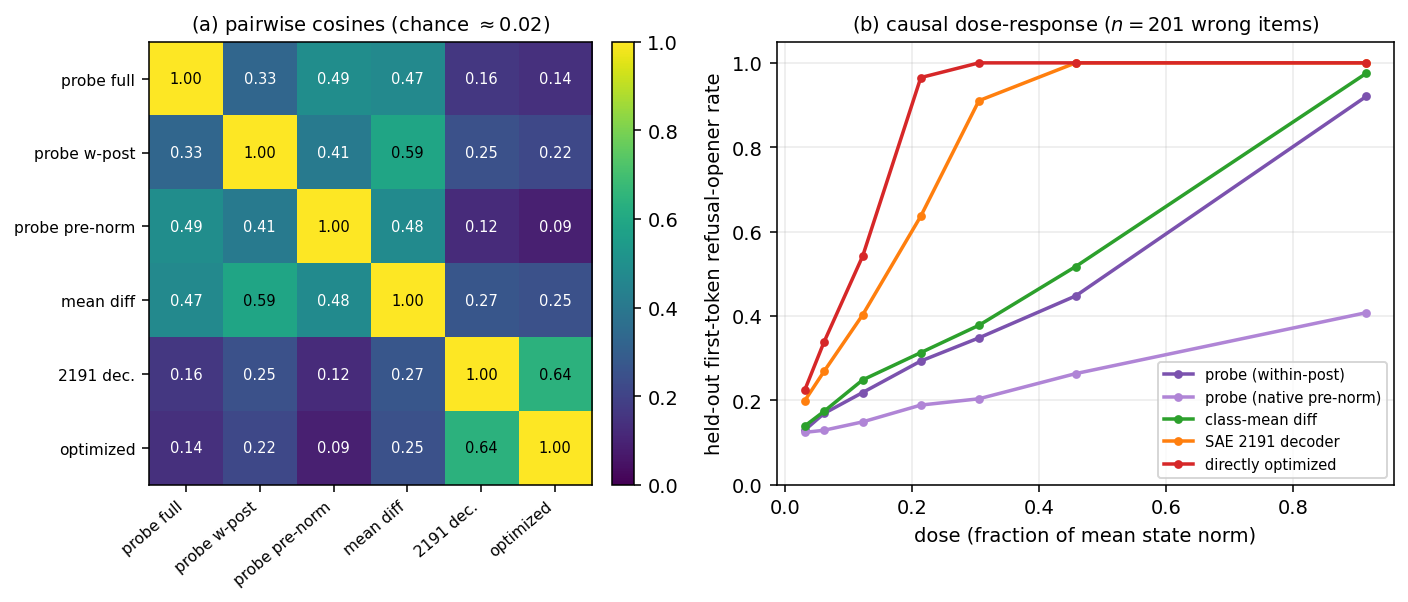
\includegraphics[width=\linewidth]{figures/qwen3_1_7b/direction_candidates.png}
\caption{The geometry of the six refusal-direction candidates.
\textbf{(a)} Pairwise cosines split the recoveries into two families:
data-side (probe variants and the class-mean difference, \(0.33\)--\(0.59\))
and output-side (2191 decoder and directly optimized, \(0.64\)),
weakly coupled (\(0.09\)--\(0.27\); chance \(\approx 0.02\) in
\(2048\)-d). \textbf{(b)} Held-out first-token flip curves, doses as
fractions of the mean state norm: causal potency tracks output-family
membership, not discriminative quality. The native pre-norm probe
separates the classes as well as any recovery (Appendix C) yet carries
the least leverage.}\label{fig:candidates}
\end{figure}

All four causal routes converge on the strict criterion: on the same
wrong items, the probe push, the 2191 push, and prefix-forcing either
literal opener produce the same downstream judged-refusal rate of
roughly one in three, consistent with complete mediation at the first
token (per-route rates, the not-powered-as-equivalence caveat, and
dose-for-dose accounting in Appendix C).

